\documentclass{article}
\usepackage[utf8]{inputenc}
\usepackage{amssymb, amsmath}
\usepackage[hidelinks]{hyperref}
\usepackage{graphicx}
\usepackage{url}
\graphicspath{ {../graphs/} }
\usepackage{listings}
\begin{document}

\title{ \textbf{\Huge Visiochess} \\
		{\large A Visual Analysis of Chess Openings Over Time}
}
\author{
Murray Heymann\\ 15988694 \and Jolandi Lombard\\ 16994914 \and Lisa van Staden\\ 18245471 \and Elan van Biljon\\ 18384439 \and Trandon Narasimulu\\ 19044186 \and Francois Kunz\\ 19163630}
\date{\today}
\clearpage\maketitle
\thispagestyle{empty} % make sure no page numbers on title page

\pagebreak

\clearpage\tableofcontents
\thispagestyle{empty}  % make sure no page numbers on title page

\pagebreak
\setcounter{page}{1} % Set the page counter to 1

\section{Specifications}
The purpose of this project is to develop a web application to provide
the user with a detailed analysis
of the popularity of chess openings over the years.

\subsection{General}
The user can view the default database or upload their own data, provided
it is in the correct file
format, PGN, and contains the needed information.The web application is
made fully responsive by using Bootstrap\cite{boot}.
A user file is restricted to a maximum size of $10$Mb ($10\ 000\ 000$ bytes)
The visual representation of the analysis is done using D3.js \cite{d3}.
The user can view all the data or apply the following filters:
\begin{enumerate}
	\item Data Range by year
	\item WhiteElo and BlackElo
    \item ECO Codes\cite{eco}:
	\begin{itemize}
		\item Primary ECO codes (A-E)
		\item ECO categories(13 categories)
		\item ECO subcategories (one of 500)
	\end{itemize}
\end{enumerate}

\subsection{Front End}
The front end shall make use of D3.js for visualization of processed data.
The front end shall give a visual summary of the information after filtering.
The front end shall have a list of databases to choose from.  The list
shall always contain the default database of the back end, along
with any databases uploaded by the user.
Before a user has uploaded any data, the default data set \cite{def_db} shall
be preselected.
Upon loading a pgn file, the newly uploaded data set shall the selected
data set.

\subsection{Back End}
The back end shall have an API for receiving an uploaded PGN file.
The back end shall parse the PGN file into a MySQL database.
The back end shall have an API for receiving filtering commands.
The back end shall process filtering commands into MySQL queries.
The back end shall perform MySQL queries on databases of chess games.
The back end shall return a JSON object with the following structure:
\begin{lstlisting}
	{
		error: boolean value
		error_message: String
		data: JSON
		pop: array
	}
\end{lstlisting}
The JSON object for the data field shall have the following structure:
\begin{lstlisting}[escapeinside={(*@}{@*)}]
	{
		year: array of values
		(*@{\vdots}@*)
	}
\end{lstlisting}

\section{Program Description}

\subsection{Back End}
The back end is comprised of all code that gets executed on the server side.

All database queries are done here, mostly because the default database is
assumed to be used most often and is found here. This also allows devices
with limited processing power to use the service with ease, while also
requiring a server with reasonably large memory, storage and
processing abilities.

\subsubsection{make.sh}
This is a Linux bash script that sets up the back end environment.
It downloads all necessary dependencies, creates the MySQL database
and creates a configuration file for the server.

\subsubsection{make\_osx.sh}
This is a OSX bash script that sets up the back end environment.
It downloads all necessary dependencies, creates the MySQL database and
creates a configuration file for the server.

\subsubsection{.my.cnf}
This is a configuration file that is generated. It contains all the
information needed to connect to the MySQL server.

\subsubsection{user\_upload.php}
As the specifications dictate that users need to be able to upload their own
custom database, user\_upload.php receives such uploads and
performs some basic checks on the uploaded file, before saving it to the
server disk. The file is hashed using sha256\cite{sha} and this hash is used
as
the file name when saved, allowing users to easily specify which file
they wish to use, while avoiding any possible clashes in the naming
domain, should different users upload different files with the same name.
Conveniently, if two users upload identical databases, these databases
won't be duplicated on the server.

After a file has been uploaded successfully, a database is created with
the same name as the local file. This is done in create\_db.php with
the function create\_database.

Once the file has been saved, it is parsed. For each game, there are
three different kinds of data to parse: the seven tags required in PGN,
optional tags and the moves made during the game. It is parsed by
using the parse\_pgn\_file function in pgn\_parser.php.

\subsubsection{create\_db.php}
This script contains a function to create a database for a newly uploaded
file. It has to parse the file to determine the string length to be stored
in the moves field. First the login details for a MySQL user is read from
a file named .my.cnf in the root directory of the project.  This is then
used to connect to the MySQL server on the local server.  Once a connection
is set up, a database is created with a query, and its success is checked.
The connection is then closed.
\begin{itemize}
	\item create\_database(\$db\_name, \$target\_file)
\end{itemize}

\subsubsection{create\_default\_db.php}
This script creates a new database into which the default data set is then
parsed. This script is run to set up the database initially.

\subsubsection{eco\_category.php}
This script provides functions to translate between ECO categories and ranges.
There are two functions in this script. The get\_eco\_category function takes
in an ECO code and returns the category containing that code. The
get\_eco\_class\_ranges returns the code ranges of the given ECO category.
\begin{itemize}
	\item get\_eco\_category(\$ECO\_alpha, \$ECO\_numero)
	\item get\_eco\_class\_ranges(\$category)
\end{itemize}
\begin{lstlisting}
Example:
get_eco_category(A, 55) will return A1.4
get_eco_class_ranges(A1.4) will return A50-A79
\end{lstlisting}

\subsubsection{has\_db.php}
This script ensures that the requested user database is present on the server.
The has\_db\_available function searches the server for the requested databse.
A boolean value is returned.
\begin{itemize}
	\item had\_db\_available(\$name)
\end{itemize}

\subsubsection{pgn\_parser.php}
This file mostly defines functions used by the user\_upload.php script.
As the name suggests, it parses PGN files. This script contains functions to
skip white spaces and empty lines. It also has a function to scan the tags
when parsing a PGN file and to get the length of the longest move string in
the PGN file. The main function in this script is the parse\_pgn\_gile\_to\_db
function. The standard seven tags as required by the PGN are processed with
the sscan\_tag function and have their values stored in local variables.
Thereafter, the optional tags are scanned and each examined as either being
an ECO tag or a black or white ELO tag.  If any of these are not present,
their local variable simply gets the empty string assigned to it.

The moves are often listed over various lines.  First, these moves are
collected into a single line string.  Then, the string is split by spaces,
to produce an array.  On array indices that are multiples of three, one
finds the move numbers.  On the very last non-trivial entry, one finds
the score of the match.  All other entries indicate moves:
\begin{align*}
\forall i \in \{ x\in \mathbb{Z}\ :\ & x\text{ a valid index in moves array}\},\\
i & \equiv 2\pmod 3 \implies \text{moves[i] denotes a black move}\\
i & \equiv 1\pmod 3 \implies \text{moves[i] denotes a white move}
\end{align*}
The moves are separated into an array of white moves and an array of black
moves. These arrays are then stored in an object than can be easily sent to
a function that will insert the data into the MySQL database.

\begin{itemize}
	\item sscan\_tag(\$read\_string, \$start\_of\_string = \textquotedblleft
	[Event \textbackslash \textquotedblleft\textquotedblright )
	\item evaluate\_line(\$line, \$should\_start)
	\item parse\_white\_space(\$db\_file, \$dud\_line)
	\item parse\_pgn\_file\_to\_db(\$target\_file, \$db\_name)
	\item get\_longest\_moves\_string(\$target\_file)
\end{itemize}

\subsubsection{query\_*.php}
This is a generic description of the query scripts that follow. The user
sends filters to be applied to the database.  These filters are sent to
query.php, which then formulates the filter data into MySQL queries.
These queries are made into the database and the results are sent back to
the user.

\subsubsection{query\_cat.php}
This script performs all queries when filtering by ECO category.

\subsubsection{query\_class.php}
This script performs all queries when filtering by ECO class.

\subsubsection{query\_code.php}
This script performs all queries when filtering by ECO code.

\subsubsection{query\_year.php}
This script performs all queries when filtering for a single given year.

\subsubsection{mysql\_interface.php}
This file contains the \texttt{ServerInterface} class. This class is a PHP
interface built on top of the \texttt{mysqli} interface. It adds another
layer of abstraction that makes interfacing with MySQL servers much easier.
\\Among others it provides functions to:
\begin{itemize}
	\item connect to a MySQL server.
	\item create, delete and use a database.
	\item create and delete a table.
	\item create and delete an index.
	\item insert data into a table.
	\item fetch data from the database (make queries).
	\item send SQL commands to the server.
\end{itemize}
Functions:
\begin{itemize}
	\item \_\_construct(\$server=null, \$user=null, \$password=null,
	\$port=null, \$verbose=false)
	\item quit(\$error\_message=\textquotedblleft\textquotedblright)
	\item connect()
	\item disconnect()
	\item attempt(\$query)
	\item create\_database(\$name=null, \$replace=false)
	\item delete\_database(\$name=null)
	\item use\_database(\$name=null)
	\item create\_table(\$name=null, \$structure=null, \$replace=false)
	\item delete\_table(delete\_table)
	\item create\_index(\$iname=null, \$tname=null, \$cols=null,
	\$replace=false)
	\item delete\_index(\$iname=null, \$tname=null)
	\item insert(\$table\_name=null, \$data=null)
	\item insert\_multiple(\$table\_name=null, \$data=null)
	\item select\_from(\$table\_name=null, \$columns=null, \$conditions=null
	\$extra\_arguments=null)
	\item sql(\$sql=null)
\end{itemize}


\subsubsection{utils.php}
The utils.php script provides utilitarian functions to prevent code
duplications. This script has functions to process ECO and year data. The
contains function checks whether a string is present in some token. The
trim\_chars function removes a given number of characters from the end of a
given string. The stringify funtion translates objects to strings. The
set\_query\_where\_fields constructs a query data structue that is sent to the
server.
\begin{itemize}
	\item contains(\$string, \$token)
	\item stringify(\$object)
	\item trim\_chars(\$string, \$num\_chars)
	\item process\_elo\_data(\$result, \&\$num\_ecos, \&\$top\_ecos,
		\&\$json\_data)
	\item process\_year\_data(\$result, \&\$num\_ecos, \&\$top\_ecos,
		\&\$json\_data)
	\item set\_query\_where\_fields(\$filter\_on, \$filters, \&\$query)
\end{itemize}

\subsubsection{validate.php}
TODO
\begin{itemize}
	\item validate\_filters(\$filters)
	\item validate\_year(\$filters, \$response=null)
	\item validate\_given\_year(\$year, \$response=null)
	\item validate\_year\_low(\$year, \$response=null)
	\item validate\_year\_high(\$year, \$response=null)
	\item validate\_elos(\$filters, \$response=null)
	\item validate\_elo(\$filters, \$type, \$response=null)
	\item validate\_elo\_low(\$filters, \$type, \$response=null)
	\item validate\_elo\_high(\$filters, \$type, \$response=null)
	\item validate\_eco(\$filters, \$response=null)
	\item validate\_eco\_cat(\$eco\_category, \$response=null)
	\item validate\_eco\_class(\$eco\_class, \$response=null)
	\item validate\_eco\_low(\$eco, \$response=null)
	\item validate\_eco\_high(\$eco, \$response=null)
	\item new\_response()
	\item add\_error(\$error, \$response=null)
	\item add\_filter(\$filter, \$response=null)
	\item low\_greater\_than\_high(\$low, \$high, \$filter, \$response=null)
\end{itemize}

\subsection{Front End}
The front end is presented to the user using HTML5 (index.html) and
supplemented with JavaScript (main.js) to allow for an interactive and
dynamic experience.  The data returned by a query to the server is
displayed using D3.js in a dedicated section.  Links to a description
of the web application (about.html) and the course
website is provided in the footer.

CSS styling is based on Bootstrap and supplemented with a custom styling
sheet (css/style.css) generated by Sass (style.scss).

\subsubsection{main.js}
This file contains the JavaScript that will run in the clients browser. It
will handle user interaction (such as constructing new filters and uploading
files). It will make the necessary ajax calls to the server when the user
wants to apply filters and upload their own PGN file. This file also
validates all user input to ensure it is correct and safe to send to the server.

\subsubsection*{add\_max\_year\_attr}
TODO

\subsubsection*{getConfigSettings}
TODO

\subsubsection*{handle\_pgn\_submit function}
This function runs some checks on the submitted PGN file and if it passes
all the checks it uses \textit{hex\_sha256.js} to hash the file. It then
sends the file and a hash of the file to the server using ajax.

\subsubsection*{submit\_file}
TODO

\subsubsection*{handle\_filter\_submit function}
This function sends the filter form data in json form to the server.
(It will handle the response properly later but for now it just embeds it into
the html)

\subsubsection*{getFormData function}
This function serializes and returns form data in the form of a json.
(I believe it was acquired from stackoverflow.com, we should reference that)

\subsubsection*{ensure\_database\_exists\_on\_server}
TODO

\subsubsection*{handle\_filter\_response}
TODO

\subsubsection*{get\_file\_from\_hash}
TODO

\subsubsection*{handle\_filter\_clear}
TODO

\subsubsection*{handle\_window\_resize}
TODO

\subsubsection*{handleEcoFilterChange}
TODO

\subsubsection{visual\_response.js}
This file contains JavaScript that will run in the clients browser. It
will handle the visualization of the data, that is received from the server
after
the filters have been submitted. A lot of the code is based on the Stacked Area
Chart Example \cite{chart}.
\begin{itemize}
	\item TODO
\end{itemize}
\subsection*{draw}
This function receives a JSON object from handle\_response or
handle\_window\_resize in main.js. After this object has
been processed, the data it contains is then visualized using the D3
library functions.

\subsubsection*{process\_JSON\_to\_D3}
This function creates and returns a new JSON object from the received
data function which will be used to create the graph.

\section{Database}
The data specified for this program is found in a file called
millionbase-2.5.pgn \cite{def_db}, which as the name suggest has 2.5 million
chess game summaries. Each one of these is put into the database as a row
containing multiple different fields.  This provided two challenges:
populating the database in a reasonable time, and getting query results as
quickly as possible.

\subsection{Design of the database}
TODO

\subsection{Populating database}
The parser started with a naive approach of putting each game into the
database as soon as it was read.  This process took 50 minutes to parse the
whole database the first time.

Although populating the database is a once
off procedure when setting up a server like this, this did pose a problem,
as there was still debugging to be done on the parser and the addition of
further parsing features to allow for minor errors in notation. Every change to
the parser required testing.  For every bug in the parsing process that leads
to a corrupt entry in the database that is corrected, the whole large database
would need to be re-parsed.  Therefore, parsing times should be improved.

It was found that adding the games to the database in batches of 1000 rows,
instead of one at a time significantly improved parsing times. By batching them
together in groups of a thousand, the database could be populated in about 5
minutes, an improvement by one order of magnitude.

The question immediately arose:  What is the optimal batch size? To set out
to answer this question, the data contained in the "tags" table was parsed in
varying batch sizes, each time measuring the time this procedure took.  A
few sample batch sizes quickly reveals that the optimal batch size for the
tags table was somewhere between 100 and 240.

Next, measurements for batch sizes between 80 and
240, taking steps of 10, was systematically taken.  For each batch size,
multiple parses were attempted and the top three results for each was noted.
This is reasonable, as we are interested in the best optimal case, not the best
average parse time for a batch size.  The results are shown in table
\ref{table:1}.

\begin{table}[h!]
	\centering
	\begin{tabular}{||c c c c||}
		\hline
		Batch Size & Measure 1 & Measure 2 & Measure 3 \\ [0.5ex]
		\hline\hline
		80 & 3:48.322 & 3:48.878 & 3:49.188 \\ [0.5ex]
		\hline
		90 & 3:42.912 & 3:43.003 & 3:43.854 \\ [0.5ex]
		\hline
		100 & 3:37.482 & 3:37.677 & 3:37.780 \\ [0.5ex]
		\hline
		110 & 3:31.704 & 3:31.781 & 3:32.665 \\ [0.5ex]
		\hline
		120 & 3:30.718 & 3:30.811 & 3:31.262 \\ [0.5ex]
		\hline
		130 & 3:27.843 & 3:28.247 & 3:28.741 \\ [0.5ex]
		\hline
		140 & 3:27.545 & 3:27.666 & 3:27.700 \\ [0.5ex]
		\hline
		150 & 3:26.064 & 3:26.490 & 3:26.805 \\ [0.5ex]
		\hline
		160 & 3:26.658 & 3:27.013 & 3:27.416 \\ [0.5ex]
		\hline
		170 & 3:25.859 & 3:25.860 & 3:26.324 \\ [0.5ex]
		\hline
		180 & 3:26.652 & 3:26.952 & 3:27.427 \\ [0.5ex]
		\hline
		190 & 3:27.345 & 3:28.474 & 3:28.544 \\ [0.5ex]
		\hline
		200 & 3:27.552 & 3:27.712 & 3:27.763 \\ [0.5ex]
		\hline
		210 & 3:28.452 & 3:28.929 & 3:29.221 \\ [0.5ex]
		\hline
		220 & 3:29.454 & 3:29.979 & 3:30.700 \\ [0.5ex]
		\hline
		230 & 3:30.577 & 3:30.894 & 3:31.414 \\ [0.5ex]
		\hline
		240 & 3:30.406 & 3:31.958 & 3:32.874 \\ [0.5ex]
		\hline
	\end{tabular}
	\caption{Time taken in seconds to parse various batch sizes to MySQL}
	\label{table:1}
\end{table}

This data was then plotted in python as a scatter plot.  The \texttt{interp1d}
module from the \texttt{scipy} library was used to find an interpolation of
the data.  The plotted data is shown in figure \ref{figure:1}

\begin{figure}[h]
	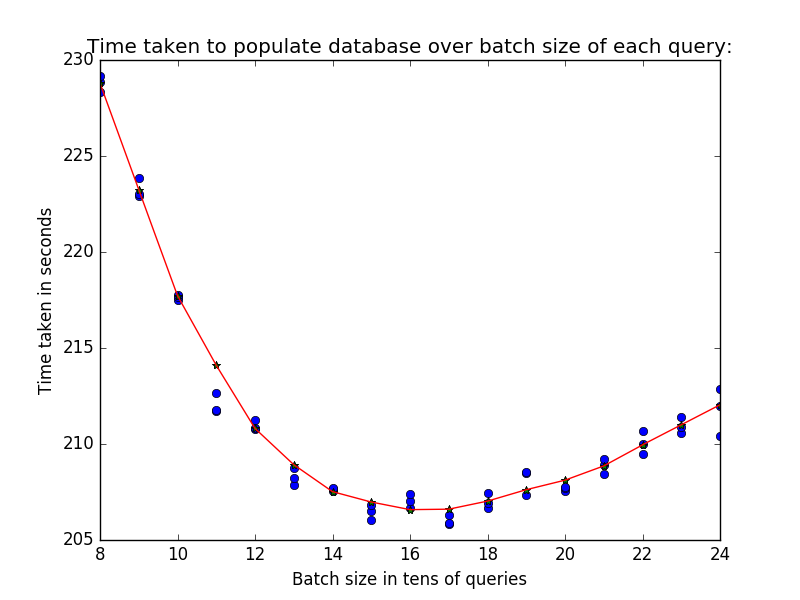
\includegraphics[width=10cm]{graph_batch_interpolation}
	\caption{Scatter plot of time taken to parse various batch sizes to
	MySQL, with the interpolated line of best fit drawn in.}
	\label{figure:1}
\end{figure}

From the graph, it seems an optimal batch size is found around when parsing
about 160 rows in a single query.

The increase in the efficiency by using batches instead of parsing single
entries lies in the overhead of PHP passing the query to MySQL.  Each
query comes with a little delay, when the text of the query is sent to the
database and again for the results that are sent back.  When entering data
one query at a time, this delay accounts for more than half of the time spent
by the parser.  When batching, say, 100 together, this overhead time stays
the same, but is divided between 100 rows.  The time taken by MySQL to
process these 100 rows might increase marginally but this is offset by the
massive reduction in overhead.

The overall time taken up by this overhead is inversely proportional to
batch size.  As batch size grows, the proportion of time spent on this
overhead tends to 0. However, this is an asymptote and will never be reached
for any real numbered batch size.  As batch size grows further, the additional
time saved in overhead diminishes, but the time taken by MySQL to process the
query grows.  Scanning of the PGN file and placing data into the database
happens synchronously, so while MySQL processes the insertion, the parser is
idling.  At some point, the time taken by the parser to wait for MySQL to
finish its insertion query starts to become significant and offsets the
gains made by reducing overhead.  Therefore, at some point, the total time
taken starts increasing again.  For our tags table, this point is reached
at about 160 rows per insertion.

\subsection{Optimization of Queries}
It made sense to try and optimize query searches.  This is done by
creating an index on each table, based on the known made queries.

Interested in the exact impact this might make on the searches, the database
was recreated without an index.  On MySQL-workbench, a graphic explanation of
how the query would be executed was found. The same query was then performed
on the database, with the index created. The average time taken to query with
an index is about 0.45 seconds, while without an index, it took about 1.1
seconds.

\begin{figure}[h]
	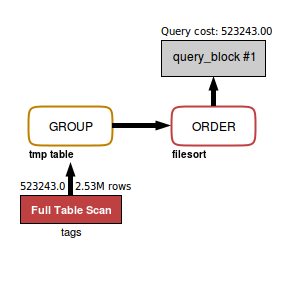
\includegraphics[width=8cm]{Query_eco_code_no_index}
	\caption{Execution of query without an index table.}
	\label{figure:2}
\end{figure}

\begin{figure}[h]
	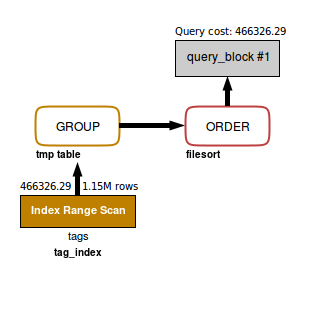
\includegraphics[width=8cm]{Query_eco_code_w_index}
	\caption{Execution of query with an index table}
	\label{figure:3}
\end{figure}

The execution graphic of the database without and index is shown in figure
\ref{figure:2}, while the graphic of the same query is shown in figure
\ref{figure:3}. The query performed looked as follows:

\begin{lstlisting}[language=sql, frame=single]
SELECT date, CONCAT(eco\_alpha, eco\_numero) as eco,
count(*) AS popularity
FROM tags
WHERE date >= 1900 AND date <= 2000 AND eco\_numero >= 10
AND eco\_numero <= 30 AND eco\_alpha = 'A'
group by eco, date
ORDER BY date, popularity DESC;
\end{lstlisting}

As expected, the query without an index table had to do a full table scan,
while the query on the indexed table had a significant reduction in the
number of rows that had to be scanned.

\section{Testing}
TODO: Used testing pyramid for reference \cite{test}
\subsection{JavaScript Testing}
For testing the JavaScript functions and functionality we used the built
in QUnit library to perform JUnit testing.

\section{Additional features}

\bibliographystyle{plain}
\bibliography{references.bib}

\end{document}
